\documentclass{article}

\newcommand{\preca}[1]{{\textsf{\small prec}@#1}}
\newcommand{\reca}[1]{{\textsf{\small recall}@#1}}
\newcommand{\ndcga}[1]{{\textsf{\small ndcg}@#1}}
\newcommand{\topk}{{\textsf{\small top}-k}}
\newcommand{\topa}[1]{{\textsf{\small top}-#1}}

\newcommand{\real}{\mathbb{R}}

\newcommand{\dsloss}{\mathsf{\small Decoupled Softmax}}
\newcommand{\stopkloss}{{\mathsf{\small SoftTop}\text{-k}}}
\newcommand{\stopat}{{\textsf{\small SoftTop}}}
\newcommand{\htopk}{{\mathsf{\small HardTop}\text{-k}}}
\newcommand{\htopat}{{\textsf{\small HardTop}}}
\usepackage[mathscr]{euscript}
\usepackage{amsfonts, bm}       % blackboard math symbols

\usepackage{setspace}
\onehalfspacing

\usepackage[left=1in, top=1in, bottom=1in, right=1in]{geometry}

\usepackage{amsmath}            % align environment

% \usepackage[compress]{natbib}
\usepackage[backend=bibtex,style=authoryear,natbib=true]{biblatex}


\usepackage{url}            % simple URL typesetting

\usepackage{graphicx}
\usepackage{float}
\addbibresource{../Reference/data.bib}
\graphicspath{{../Images/}}
\nocite{*}


\begin{document}

\vspace{-8pt}
\section{Background: multi-label classification}
\label{sec:bg}
\vspace{-5pt}
%\subsection{Multi-label classification}

As discussed in Section, the  
\begin{figure}[H]
    \centering
    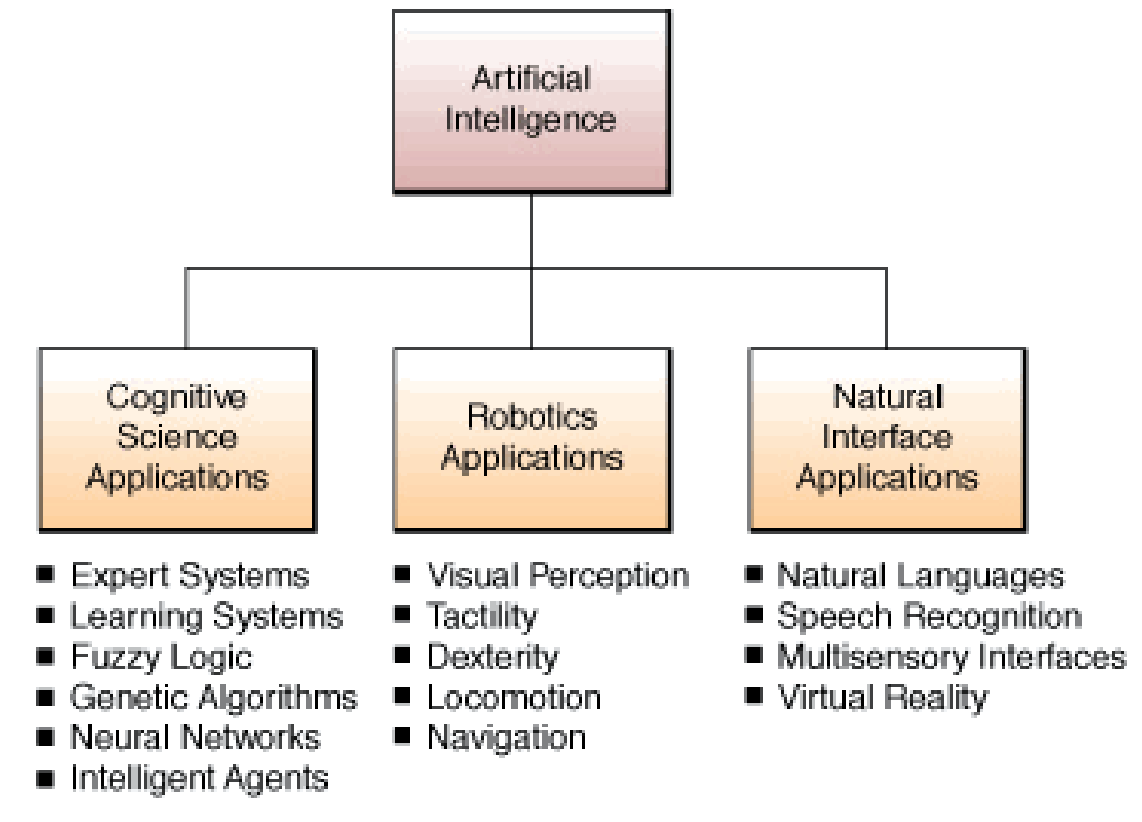
\includegraphics[width=6cm]{ai-overview.png}
    \caption{Overview of Artificial Intelligence}
    \label{fig:ai-overview}
\end{figure}

% The 
(many-shot) retrieval problem %that we 
explored in this work is essentially a multi-label classification problem. Assuming that $\mathscr{Q}$ and $\mathscr{D}$ denote the query and document (or label) spaces, respectively, the underlying \textit{query-document relevance} is defined by the distribution $\mathsf{P}$ where $\mathsf{P}(d|q)$ captures the true relevance for the query-document pair $(q, d) \in \mathscr{Q} \times \mathscr{D}$. In this paper, we assume that the document space is finite with a total $|\mathscr{D}| =  L$ documents. Let the training data consists of $N$ examples $\mathcal{S} := \{(q_i, \mathbf{y}_i)\}_{i \in {N}} \subseteq \mathscr{Q} \times \{0, 1\}^{L}$, where, for $j \in [L]$, $y_{i, j} = 1$ \textit{iff} $j$th document in $\mathscr{D}$ is relevant for query $q_i$. We also denote the set of positive labels for $q_i$ as $P_i = \{j: y_{i,j}=1\}$ %\sout{Alternatively, binary label vector $\mathbf{y}_i$ can be represented as a set $\mathcal{D}_i := \mathcal{D}_{q_i}\subset \mathscr{D}$ which has $\mathbf{y}_i$ as its indicator vector.}

\textbf{Dual-encoder models and classification networks.}~Note that learning a retrieval model is equivalent to learning a \textit{scoring function} (or simply \textit{scorer}) $s_{\bm{\theta}}: \mathscr{Q} \times \mathscr{D} \to \real$, which is parameterized by model parameters $\bm{\theta}$. A DE model consists of a \textit{query encoder} $f_{\bm{\phi}}: \mathscr{Q} \to \real^d$ and a \textit{document encoder} $h_{\bm{\psi}}: \mathscr{D} \to \real^d$ that map query and document features to $d$-dimensional embeddings, respectively. Accordingly, the corresponding scorer %functions 
for the DE model is defined as: $s_{\bm{\theta}}(q, d) = \langle x_q, z_d \rangle = \langle f_{\bm{\phi}}(q), h_{\bm{\psi}}(d) \rangle,$
% \begin{align}
% s_{\bm{\theta}}(q, d) = \langle f_{\bm{\phi}}(q), h_{\bm{\psi}}(d) \rangle,\label{eq:score-qd}
% \end{align}
where $\bm{\theta} = [\bm{\phi}; \bm{\psi}]$ and $x_q, z_d \in \real^d$. 
{Note that it is common to share encoders for query and document, i.e., $\bm{\phi} = \bm{\psi}$. We also focus on this shared parameter setting in our exploration.} %\todong{Maybe we should say that its common to share the same parameters for $\phi$ and $\psi$, and we also share the parameters in our experiments. *AR*: Done. Please take a look.}. 
%On the other hand, 

Different from DE models, classification networks ignore document features. Such networks consist of a query encoder $g_{\bm{\phi}}: \mathscr{Q} \to \real^d$ and a classification matrix $W \in \real^{L \times d}$, with $i$th row as the classification weight vector for the $i$th document. %Now the scoring function 
The scorer for the classification network then becomes $s_{\bm{\theta}}(q,d) = \langle g_{\bm{\phi}}(q), \mathbf{w}_d \rangle,$
% \begin{align}
% s_{\bm{\theta}}(q,d) = \langle g_{\bm{\phi}}(q), \mathbf{w}_d \rangle,
% \end{align}
where $\mathbf{w}_d $ denotes the classification vector associated with document $d$ and $\bm{\theta} = [\bm{\phi}; W]$. For ease of exposition, we do not always highlight the explicit dependence on trainable parameters $\bm{\theta}, \bm{\phi}, \bm{\psi}$ while discussing DE models and classification networks.

% \textbf{Performance metrics and loss functions.}\todoasr{This needs more work.}~
\textbf{Loss functions.}~
%Ideally, for a query, a scorer function would provide higher score to the relevant documents; as a result, for $k \geq 1$, $\mathsf{Top}_{k}(q; s)$ -- the set of $k$ documents with the highest scores for the query $q$ according to the scorer $s$ -- forms a natural candidate for $k$ retrieved documents. \textit{Precision-at-k} (\preca{k}) and \textit{Recall-at-k} (\reca{k}) are two widely popular metrics to assess the performance of a scorer: \sri{I think we can remove the precision and recall defintions here as we define them in experiments section. *AS:* Will remove these shortly.}
% \begin{align}
% \preca{k}(s) &:= \mathbb{E}_{(q, \mathcal{D}_q)}\left[\vert \mathcal{D}_q \cap \mathsf{Top}_{k}(q; s) \vert / k \right], \\
% \reca{k}(s) &:= \mathbb{E}_{(q, \mathcal{D}_q)}\left[\vert \mathcal{D}_q \cap \mathsf{Top}_{k}(q; s) \vert / \vert \mathcal{D}_q \vert \right].
% \end{align}
% Accordingly, 
Given the training set $\mathcal{S}$, one learns a scorer by minimizing the following objective: % typically optimizes the following training objective to learn a scorer: 
% \todoasr{Simplify the notation and make it consistent.}
\begin{align}
% R(s; \mathcal{S}) = \frac{1}{N}\sum_{i \in [N]} \ell(\mathbf{y}_i, \mathbf{s}_{q_i}),
\mathcal{L}(s; \mathcal{S}) = \frac{1}{N}\sum\nolimits_{i \in [N]} \ell(q_i,\mathbf{y}_i; s),
\end{align}
where $\ell$ is a \textit{surrogate loss-function} for some specific metrics of interest (e.g., Precision@k and Recall@k). Informally, $\ell(q, \mathbf{y}; s)$ serves as a proxy of the quality of scorer $s$ for query $q$, as measured by that metric with $\mathbf{y}$ as ground truth labels.
%where, for $q \in \mathscr{Q}$, the vector $\mathbf{s}_{q} \in \real^L$ consists of the scores assigned by $s$ to $L$ documents; and $\ell: \{0, 1\}^L \times \real^L \to \real$ is a \textit{surrogate loss-function} for the metrics of interest (e.g., \preca{k} or \reca{k}).
One of the popular loss functions for multi-label classification problem is obtained by employing one-vs-all (OvA) reduction to convert the problem into $L$ binary classification tasks~\citep{lapin2016topk}. Subsequently, we can invoke a binary classification loss such as sigmoid \textit{binary cross-entropy} (BCE) for $L$ tasks, which leads to OvA-BCE:
\begin{align}
\label{eq:bce-ova}
% \ell(q, \mathbf{y}, s) = \sum\nolimits_{j \in [L]}\log\big(1 + \exp(-y_j\exp(s(q, d_j))\big).
\ell(q, \mathbf{y}, s) =  - \sum\nolimits_{j \in [L]} \Big( y_j \cdot \log\frac{e^{s(q,d_j)}}{1 + e^{s(q,d_j)}} + (1- y_j) \cdot \log \frac{1}{1 + e^{s(q,d_j)}} \Big).
\end{align}
Alternatively, one can employ a multi-label to multi-class reduction~\citep{menon2019reduction} %\citep[see, e.g.,][and references therein]{lapin2016topk, reddi19snm, menon2019reduction} 
and invoke softmax cross-entropy (SoftmaxCE) loss for each positive label: 
% \devvrit{DK: We've been using $l(q_i, y_i, s)$ so far, for example i eq.3 as well. So better to keep that }
\begin{align}
\label{eq:sce-pal}
\ell(q, \mathbf{y}, s) =  - \sum\nolimits_{j \in [L]}y_{j}\cdot{\log \Big({e^{s(q, d_j)}}/{\sum\nolimits_{l \in [L]} e^{s(q, d_{l})}}\Big)}.
\end{align}

Our empirical findings in Section reveal that DE models fail to train with BCE loss. We hypothesize that this might be due to the stringent demand of the BCE loss, which requires all negative pairs to exhibit high absolute negative similarity and all positive pairs to have a high absolute positive similarity – a feat that can be challenging for DE representations. In the section below we analyze SoftmaxCE loss (an extreme case of InfoNCE) in more detail and highlight its shortcomings.

%See \citet{menon2019reduction} for more details on such reductions where \eqref{eq:sce-pal} is referred as Pick-all-labels (PAL) reduction.
%This \eqref{eq:sce-pal} is referred as Pick-all-labels (PAL) reduction~\citep{menon2019reduction}.

\iffalse
Note that for the \textit{multi-class} classification setting where each query has a single relevant document, i.e., $|\mathcal{D}_q| = 1 $, these metrics reduce to the \topa{$k$} accuracy~\citep{lapin2016topk}. This has prompted application of various surrogate loss function for \topa{$k$} error to train retrieval models after employing a \textit{multi-label to multi-class reduction}~\citep[see, e.g.,][and references therein]{lapin2016topk, reddi19snm, menon2019reduction}. \textit{Softmax-cross entropy} loss is a widely popular choice, which takes the following form for a given relevant query-document pair (q, d):\todoasr{Keep only discussion on PAL and OVA here.}
\begin{align}
\label{eq:sce}
\ell(d, \mathbf{s}_q) = - \sum\nolimits_{j \in [L]}y_{ij}\cdot{\log \frac{e^{s(q_i, d_j)}}{\sum_{l \in [L]} e^{s(q_i, d_{l})}}}.
\end{align}
Interestingly, softmax-cross entropy loss in \eqref{eq:sce} is known to be calibrated for \topa{$k$} error, for any $k \geq 1$. 

Alternatively, one could convert the underlying classification problem into $L$ binary classification problems and invoke, among other choices, \textit{binary cross-entropy} loss function as follows:
\begin{align}
\label{eq:bce-ova}
\ell(\mathbf{y}, \mathbf{s}_q) = \sum_{j \in [L]}\log\big(1 + \exp(-y_j\exp(s(q, d_j))\big).
\end{align}
\fi

\printbibliography


\end{document}